\documentclass[12pt,a4paper]{ctexart}

\usepackage{amsmath,amssymb}
\usepackage{booktabs}
\usepackage{enumitem}
\usepackage{float}
\usepackage{geometry}
\usepackage{graphicx}
\usepackage{hyperref}
\usepackage{longtable}
\usepackage{tabularx}
\usepackage{xcolor}

\geometry{top=2.54cm,bottom=2.54cm,left=3.175cm,right=3.175cm}
\setlength{\parindent}{2em}
\setlength{\parskip}{0pt}
\renewcommand{\arraystretch}{1.25}
\hypersetup{colorlinks=true,linkcolor=black,urlcolor=blue}

\newcommand{\blankline}[1]{\rule{#1}{0.4pt}}

\begin{document}

\begin{titlepage}
  \noindent 组号：\blankline{3.5cm}

  \vspace{1.8cm}
  \begin{center}
    
\includegraphics[width=6.1cm]{figures/zju_logo.png}

    \vspace{1.1cm}
    {\heiti\Large 本科实验报告}

    \vspace{2.3cm}
    \begin{tabular}{rl}
      课程名称： & 机器人与智能系统综合实践\\[0.55cm]
      姓\hspace{2em}名： & 刘峻豪\quad 莫移合\quad 蓝恩先\\[0.55cm]
      院\hspace{2em}系： & 控制学院\\[0.55cm]
      专\hspace{2em}业： & 控制自动化\\[0.55cm]
      学\hspace{2em}号： & 3230105220\quad 3230102397\quad 3230104940\\[0.55cm]
      指导老师： & 任沁源\quad 姚近科\\[0.55cm]
      选课时间： & \blankline{6.0cm}
    \end{tabular}

    \vfill
    \blankline{1.2cm} 年 \blankline{0.8cm} 月 \blankline{0.8cm} 日
  \end{center}
\end{titlepage}

\newpage
\begin{center}
  
\includegraphics[width=4.2cm]{figures/zju_logo.png}
  {\heiti\LARGE 实验报告}
\end{center}

\noindent
\begin{tabularx}{\textwidth}{Xr}
  & 专业：控制自动化\\
  & 姓名：刘峻豪\quad 莫移合\quad 蓝恩先\\
  & 学号：3230105220\quad 3230102397\quad 3230104940\\
  & 日期：\blankline{2.2cm}\\
  & 地点：\blankline{2.2cm}\\
\end{tabularx}

\noindent 课程名称：机器人与智能系统综合实践
\hfill 指导老师：任沁源\quad 姚近科
\hfill 成绩：\blankline{1.5cm}

\noindent 实验名称：TurtleBot4 移动机器人自主导航与避障
\hfill 实验类型：综合性实验

\noindent 同组学生姓名：刘峻豪\quad 莫移合\quad 蓝恩先

\vspace{0.35cm}
\begin{tabularx}{\textwidth}{X X}
  一、实验目的和要求（必填） & 二、实验内容和原理（必填）\\
  三、主要仪器设备（必填） & 四、操作方法和实验步骤\\
  五、实验数据记录和处理 & 六、实验结果与分析（必填）\\
  七、讨论、心得 & \\
\end{tabularx}

\section*{一、实验目的和要求（必填）}

\subsection*{1.1 实验目的}

本实验以 TurtleBot4 移动机器人为对象，综合使用 ROS 2 Humble、Ignition
Gazebo、RViz、SLAM Toolbox、AMCL 和 Nav2，完成从环境感知、地图表达、机器人
定位、全局路径规划到闭环运动控制的完整自主导航流程。实验重点不是仅在 RViz
中画出一条路径，而是验证自研 A* 全局规划器确实被 Nav2 动态加载，并由同一条
\texttt{NavigateToPose} action 驱动机器人绕过货架到达目标。

实验由两部分组成：
\begin{enumerate}[label=\arabic*)]
  \item \textbf{计算机仿真部分：}在 warehouse 世界中，以红点
  $(-11.25,-10.50)$ 为起点、蓝点 $(0.40,-10.50)$ 为目标，完成跨越两组货架的
  长距离绕行，并对路径几何、定位稳定性、仿真时钟、规划器加载状态、action
  终态和完整视频进行量化验收。
  \item \textbf{实地实验部分：}将同一 ROS 2 包、A* 插件和 Nav2 参数迁移到实体
  TurtleBot4，在 Ubuntu 22.04 和 ROS 2 Humble 环境下完成实地 SLAM 增量建图、
  地图保存与自主导航。实地过程整体进展顺利，机器人成功完成建图与导航，并以连续
  录像和保存的栅格地图作为佐证。本部分以视频与地图作为辅助说明，量化验收指标以
  仿真部分为主。
\end{enumerate}

\subsection*{1.2 实验要求}

\begin{enumerate}[label=\arabic*)]
  \item 调用 SLAM 或课程提供的匹配地图建立导航所需的占据栅格地图；
  \item 使用 AMCL 和 TF 在 \texttt{map} 坐标系下获得机器人稳定姿态；
  \item 编程实现全局路径规划算法，并按
  \texttt{nav2\_core::GlobalPlanner} 接口接入 Planner Server；
  \item 设置明确起点和目标点，使机器人在仿真环境中自主绕障；
  \item 使用路径长度、绕行比、横向偏移和直线障碍段数证明路线具有足够难度；
  \item 保存原始路径、日志、JSON、时钟、定位、视频元数据和运行截图；
  \item 在实体 TurtleBot4 上完成实地建图与自主导航，保存栅格地图与连续录像作为佐证。
\end{enumerate}

\section*{二、实验内容和原理（必填）}

\subsection*{2.1 系统总体架构}

图 1 给出仿真系统的数据与控制链。Gazebo 提供机器人模型、
RPLIDAR、里程计和仿真时钟；SLAM Toolbox 或 Map Server 提供地图；AMCL 根据
LaserScan 与静态地图计算 \texttt{map -> odom}；Nav2 的 BT Navigator 接收目标，
Planner Server 调用自定义 A* 插件生成全局路径，DWB Controller 计算局部速度，
Velocity Smoother 将 \texttt{/cmd\_vel\_nav} 平滑为底盘执行的 \texttt{/cmd\_vel}。

\begin{figure}[H]
  \centering
  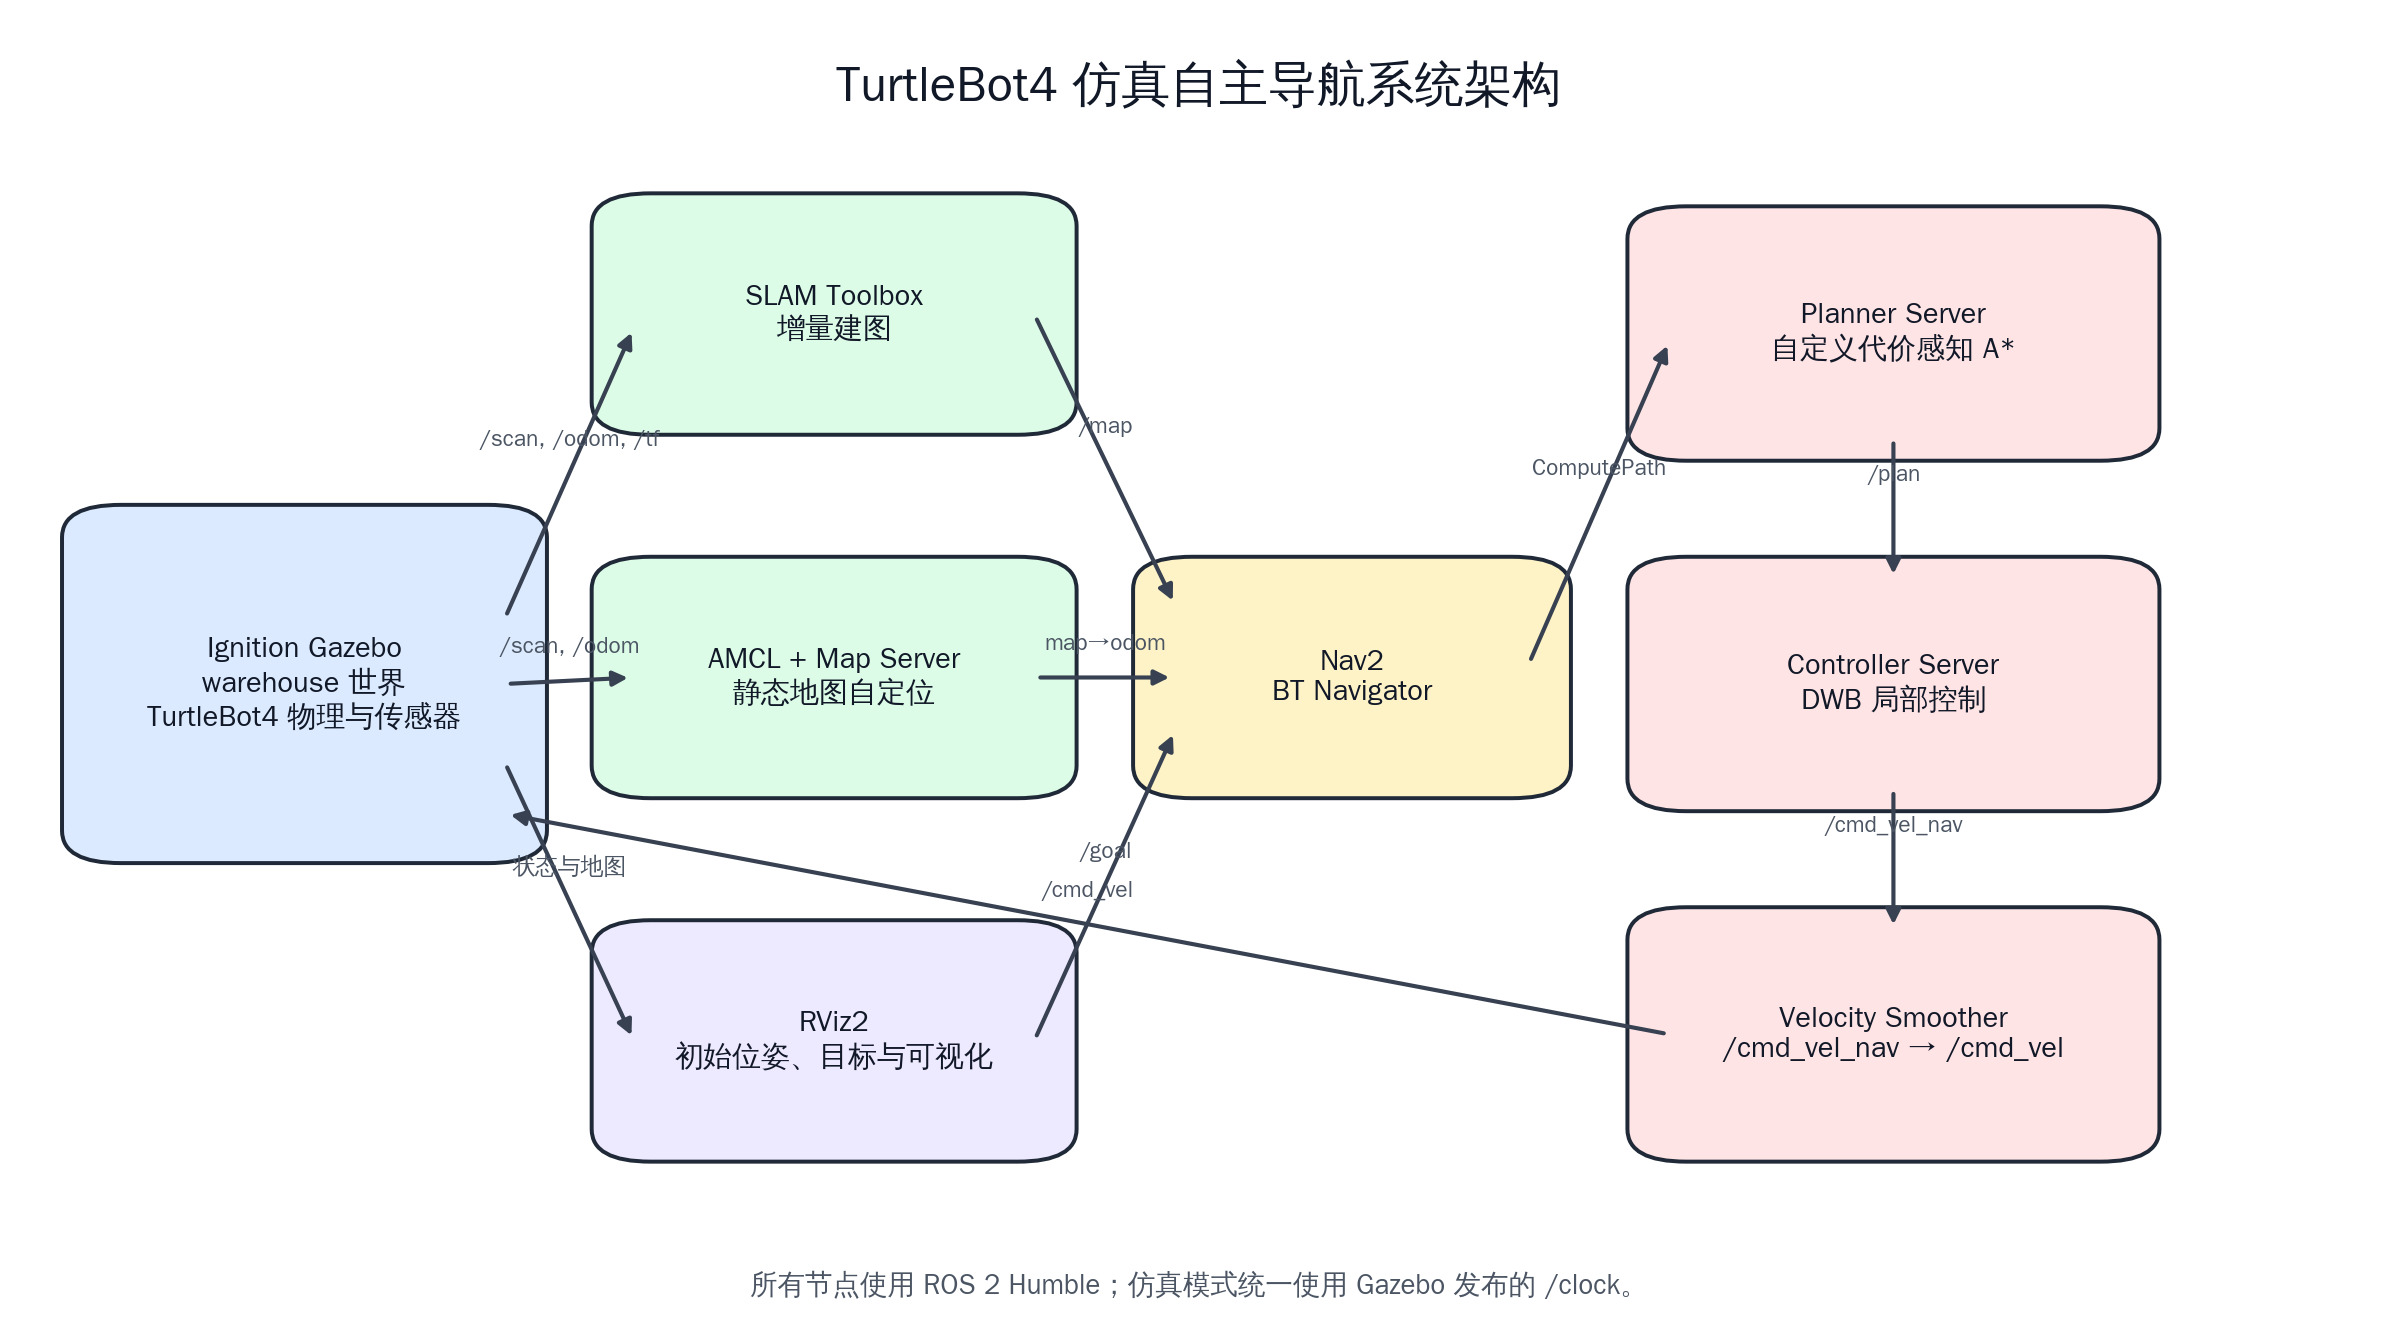
\includegraphics[width=\textwidth]{figures/system_architecture.png}
  \caption{图 1：TurtleBot4 仿真自主导航系统架构}
\end{figure}

\subsection*{2.2 差速底盘与坐标变换}

TurtleBot4 的平面位姿记为 $\mathbf{x}=[x,y,\theta]^{T}$。线速度为 $v$、角速度为
$\omega$ 时，其运动学模型为
\begin{equation}
  \dot{x}=v\cos\theta,\qquad
  \dot{y}=v\sin\theta,\qquad
  \dot{\theta}=\omega .
\end{equation}
导航使用 \texttt{map}、\texttt{odom} 和 \texttt{base\_link} 三层坐标系。AMCL 发布
\texttt{map -> odom}，底盘里程计发布 \texttt{odom -> base\_link}，因此目标点、全局
路径与机器人实时位置能够统一到地图坐标系。

\subsection*{2.3 AMCL 与 LaserScan 地图匹配}

AMCL 以粒子集合表示机器人位姿后验概率。运动模型根据里程计传播粒子，观测模型
根据激光端点与占据栅格的一致性更新权重。本实验在发送导航目标前连续观察
\texttt{map -> base\_link}，并将 LaserScan 端点投影到地图，计算位置漂移、航向漂移
和占用栅格匹配率。只有稳定性检查通过后才启动长距离 action，避免将初始化错误
误认为规划或控制故障。

\subsection*{2.4 代价感知 A* 全局路径规划}

地图被离散为二维栅格。对任意候选节点 $n$，A* 使用
\begin{equation}
  f(n)=g(n)+h(n),
\end{equation}
其中 $g(n)$ 为起点到 $n$ 的累计代价，$h(n)$ 为 $n$ 到目标的启发式估计。程序在
八连通栅格上使用 octile distance：
\begin{equation}
  h(n)=\max(\Delta x,\Delta y)
  +(\sqrt{2}-1)\min(\Delta x,\Delta y).
\end{equation}

为避免路径贴近障碍，移动到栅格 $c$ 的代价定义为
\begin{equation}
  C(c)=d\left(1+\lambda\frac{\min(\mathrm{cost}(c),252)}{252}\right),
\end{equation}
其中 $d$ 为直移或斜移距离，$\lambda=2.0$ 为代价惩罚系数。规划器将
\texttt{cost >= 253} 的栅格视为不可通行，禁止进入未知区域，并在对角移动前检查
两个正交相邻栅格，从而避免穿过被阻塞的拐角。

插件类实现 \texttt{configure}、\texttt{activate}、\texttt{deactivate}、
\texttt{cleanup} 和 \texttt{createPlan} 生命周期接口。Planner Server 通过
pluginlib 名称 \texttt{tb4\_astar\_planner/AStarPlanner} 动态加载该类，并使用
\texttt{GridBased} 作为默认 planner ID。

\subsection*{2.5 Nav2 闭环导航}

BT Navigator 的默认行为树周期性请求全局路径并调用 DWB 跟踪。全局代价地图融合
静态地图、激光障碍层和膨胀层；局部代价地图使用滚动窗口实时处理近场障碍。
本实验的机器人半径为 $0.175$ m、膨胀半径为 $0.45$ m、最大前进速度为
$0.26$ m/s。action 只有在目标检查器确认机器人位于目标容差内时才返回
\texttt{SUCCEEDED (4)}。

\subsection*{2.6 红蓝点路线的量化验收}

起点 $S$ 与目标 $G$ 的直线距离为
\begin{equation}
  D=\lVert G-S\rVert_2 .
\end{equation}
路径相邻位姿欧氏距离之和为
\begin{equation}
  L=\sum_{i=1}^{N-1}\lVert P_{i+1}-P_i\rVert_2 .
\end{equation}
绕行比定义为 $R=L/D$。最大横向绕行量为所有路径点到直线
$\overline{SG}$ 的最大垂直距离。运行器还沿起终点直线采样地图，统计连续占用
栅格形成的独立障碍段数。验收门槛分别为 $L\geq22$ m、$R\geq1.8$、横向绕行
$\geq6$ m、直线障碍段数 $\geq2$，并要求同一 action 最终成功。

\section*{三、主要仪器设备（必填）}

\begin{longtable}{p{3.2cm}p{10.6cm}}
  \toprule
  项目 & 配置或用途\\
  \midrule
  \endhead
  操作系统 & Ubuntu 22.04 LTS，ROS 2 Humble Hawksbill\\
  仿真平台 & Ignition Gazebo / TurtleBot4 warehouse 世界\\
  可视化工具 & RViz2，显示地图、机器人、LaserScan、AMCL、全局路径和代价地图\\
  建图与定位 & SLAM Toolbox、Nav2 Map Server、AMCL、TF2\\
  导航框架 & BT Navigator、Planner Server、DWB Controller、Velocity Smoother\\
  全局规划器 & 自研 \texttt{tb4\_astar\_planner/AStarPlanner} C++ pluginlib 插件\\
  自动验收工具 & \texttt{validate\_localization\_stability}、
  \texttt{run\_long\_navigation}、\texttt{ros2 topic hz /clock}\\
  测试计算机 & VMware 虚拟机，约 6 vCPU、7.7 GiB 内存、无独立 GPU\\
  实地设备 & 实体 TurtleBot4、RPLIDAR 激光雷达、充电底座、无线网络与远程主机，
  用于实地 SLAM 建图与自主导航\\
  \bottomrule
\end{longtable}

\section*{四、操作方法和实验步骤}

\subsection*{4.1 编译工作空间}

在 ROS 2 Humble 环境中安装依赖并构建：
\begin{verbatim}
source /opt/ros/humble/setup.bash
cd experiment2/ros2_ws
rosdep install --from-paths src --ignore-src -r -y
colcon build --symlink-install
source install/setup.bash
colcon test
colcon test-result --verbose
\end{verbatim}

\subsection*{4.2 启动低负载仿真与定位}

VMware 环境使用项目提供的低负载入口。该入口保留 RPLIDAR、底盘控制、里程计和
TF，关闭本次导航不需要的高负载传感器，并将 Gazebo 设为 server-only 软件渲染：
\begin{verbatim}
ros2 run tb4_experiment_bringup vmware_simulation \
  start_nav2:=false \
  x:=-11.25 y:=-10.5 yaw:=0.0 \
  localization_params:=.../localization_obstacle_route.yaml
\end{verbatim}

世界加载完成后，先验证 \texttt{/clock}、\texttt{/scan}、静态地图和
\texttt{map -> base\_link}。启动期间出现过一次仅限初始化阶段的 \texttt{/clock}
间隙，因此本次实验没有直接使用启动瞬间数据，而是在加载完成后重新采样四个时钟
窗口。

\subsection*{4.3 验证定位与 Nav2 前置条件}

\begin{verbatim}
ros2 run tb4_experiment_bringup validate_localization_stability
ros2 lifecycle get /planner_server
ros2 lifecycle get /controller_server
ros2 lifecycle get /bt_navigator
ros2 param get /planner_server GridBased.plugin
\end{verbatim}

定位检查要求连续 15 s 内位置和航向稳定，并验证 LaserScan 端点与地图占用区域
匹配。随后确认三个 Nav2 lifecycle 节点均为 \texttt{active [3]}，并确认
\texttt{GridBased.plugin} 为自定义 A*。

\subsection*{4.4 发送红点至蓝点长距离目标}

\begin{verbatim}
ros2 run tb4_experiment_bringup run_long_navigation \
  --x 0.4 --y -10.5 --yaw 0.0 \
  --min-path-length 22.0 \
  --min-detour-ratio 1.8 \
  --min-lateral-deviation 6.0 \
  --min-direct-obstacles 2 \
  --timeout 1800 \
  --evidence "$HOME/red-blue-navigation.json"
\end{verbatim}

运行器订阅 \texttt{/plan} 与 \texttt{/map}，保存目标、路径位姿数、路径长度、直线距离、
绕行比、横向绕行、障碍段数、墙钟时长和 action 终态。实验同时保存完整
\texttt{/plan} YAML、终端日志、定位日志、时钟日志和视频元数据。

\subsection*{4.5 连续视频与截图记录}

完整视频从发送目标前开始，到机器人到达蓝点并显示 action 终态后结束。视频由原始
录制片段以 stream copy 方式连接，并复用字幕流；验收不使用录制工具生成的
40.709 s 浓缩摘要，而使用 1336.604 s 的原速连续版本。关键时刻包括红点定位、
路径生成、绕过第一组货架、绕过第二组货架和蓝点 \texttt{SUCCEEDED}。

\subsection*{4.6 实地建图与实机导航}

实地实验将同一 ROS 2 工作空间部署到实体 TurtleBot4（Ubuntu 22.04、ROS 2
Humble）。整体流程进展顺利，主要步骤如下：
\begin{enumerate}[label=\arabic*)]
  \item 检查机器人电量、急停、底盘、轮胎与激光雷达，确认 \texttt{/scan}、
  \texttt{/odom}、TF 与 \texttt{/cmd\_vel} 正常；
  \item 启动 SLAM 并以低速遥控机器人沿实验场地行走，实时观察 RViz 中地图随
  激光扫描增量扩展；
  \item 使用 \texttt{map\_saver\_cli} 保存增量地图（见图 2）；
  \item 加载保存的地图，通过 AMCL 完成 \texttt{map -> odom} 定位，在 RViz 中
  确认红色激光与地图轮廓贴合；
  \item 设置目标点，由 Nav2 调用自研 A* 规划器生成全局路径并驱动机器人自主
  导航，全过程连续录像保存。
\end{enumerate}

实地建图与导航过程整体顺利，机器人成功建立场地栅格地图并完成自主移动。图 2
为实地 SLAM 过程中保存的占据栅格地图，作为实地建图的辅助说明。

\begin{figure}[H]
  \centering
  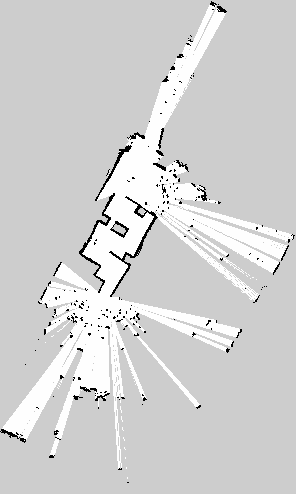
\includegraphics[width=0.6\textwidth]{figures/real_robot_map.png}
  \caption{图 2：实地 SLAM 增量建图保存的占据栅格地图}
\end{figure}

图中黑色像素为激光探测到的墙体与障碍边界，中部可辨识出结构清晰的房间与走廊
轮廓；白色为已确认的可通行区域，放射状白色扇形对应机器人所在位置的激光扫描
范围；灰色为尚未探测的未知区域。该地图为实地建图过程中的阶段性成果，配合连续
导航录像共同佐证实地实验的完成情况。

\section*{五、实验数据记录和处理}

\subsection*{5.1 原始证据清单}

\begin{longtable}{p{5.5cm}p{8.3cm}}
  \toprule
  文件 & 内容\\
  \midrule
  \endhead
  \texttt{red-blue-plan-20260715-024010.yaml} & 787 个位姿组成的完整
  \texttt{/plan} 原始消息\\
  \texttt{red-blue-navigation-20260715-024010.json} & 目标、路径几何、门槛、
  action 时长和终态\\
  \texttt{red-blue-navigation-20260715-024010.log} & goal accepted、路径指标和
  \texttt{[PASS]} 终端记录\\
  \texttt{red-blue-nav2-preconditions.log} & 自定义规划器参数以及 planner、
  controller、BT navigator lifecycle 状态\\
  \texttt{red-blue-localization.log} & AMCL/TF/LaserScan 稳定性断言\\
  \texttt{red-blue-clock-stability.log} & 世界加载后的四个 \texttt{/clock} 频率窗口\\
  \texttt{red-blue-video-ffprobe.json} & 完整视频编码、帧率和时长\\
  \texttt{test-report.md} & 完整断言、限制说明与关键截图索引\\
  \texttt{maps/real\_robot\_map.pgm} & 实地 SLAM 增量建图保存的占据栅格地图\\
  \texttt{video/实验二-实地导航.mp4} & 实地建图与自主导航连续录像\\
  \bottomrule
\end{longtable}

\subsection*{5.2 路径数据独立复算}

报告生成脚本重新读取 YAML 中全部位姿，并独立计算路径长度、直线距离、绕行比和
最大横向偏移。复算结果与 JSON 在 $10^{-9}$ 精度内一致：

\begin{longtable}{p{4.8cm}p{3.0cm}p{3.0cm}p{2.2cm}}
  \toprule
  指标 & 实测值 & 门槛 & 判定\\
  \midrule
  \endhead
  路径位姿数量 & 787 & --- & 有效\\
  路径长度 & 24.488843 m & $\geq22.0$ m & 通过\\
  起终点直线距离 & 11.650000 m & --- & 有效\\
  绕行比 & 2.102047 & $\geq1.8$ & 通过\\
  最大横向绕行 & 7.055000 m & $\geq6.0$ m & 通过\\
  直线占用区段数 & 4 段 & $\geq2$ 段 & 通过\\
  action 墙钟时长 & 1248.075 s & 记录项 & 成功返回\\
  action 终态 & SUCCEEDED (4) & 必须成功 & 通过\\
  \bottomrule
\end{longtable}

需要说明的是，1248.075 s 是低负载 VMware 仿真的墙钟时长。Gazebo 以低实时因子
运行，因此该数值不能直接代表机器人在默认物理配置或实体平台上的导航效率。

\subsection*{5.3 路径几何结果}

\begin{figure}[H]
  \centering
  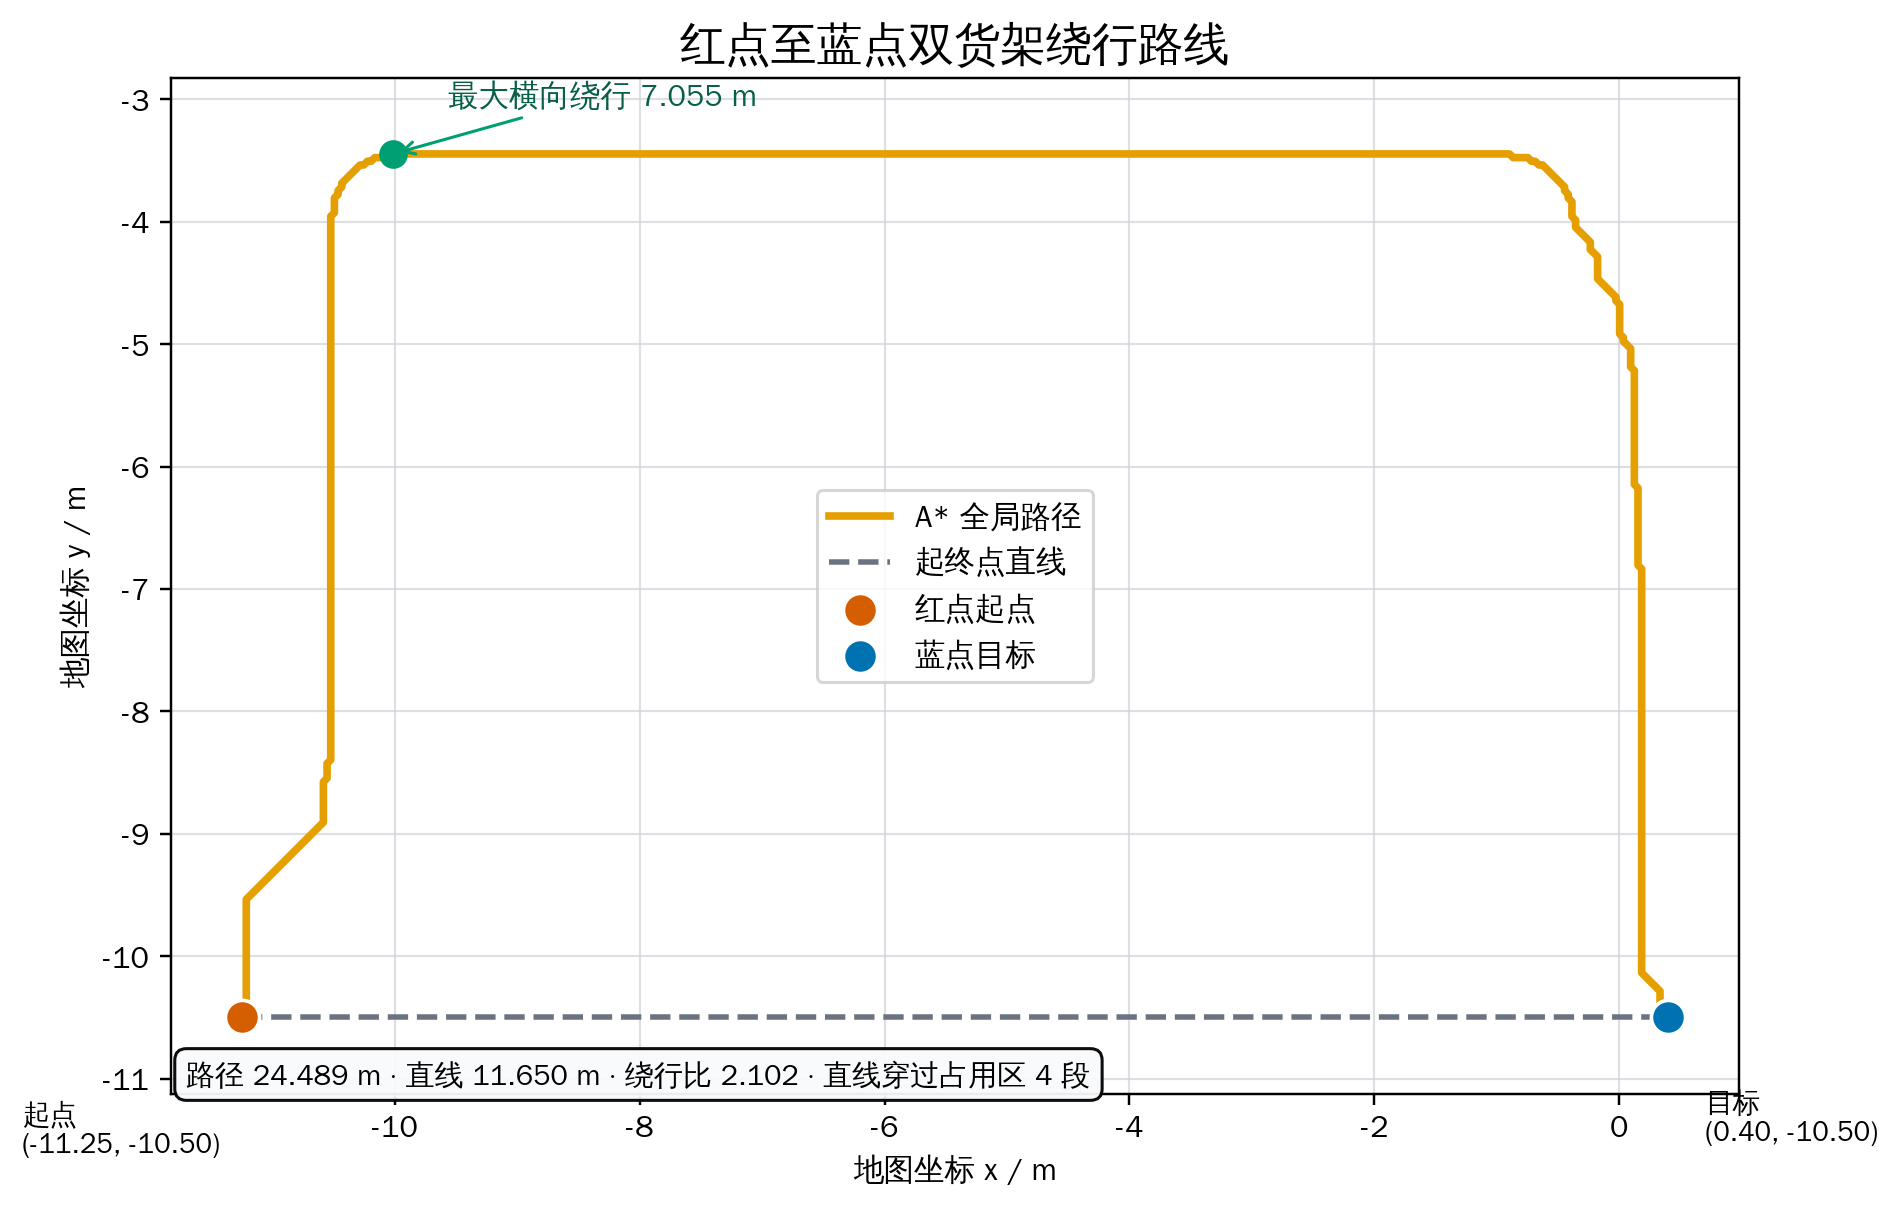
\includegraphics[width=\textwidth]{figures/red_blue_route.png}
  \caption{图 3：根据完整 YAML 路径复算的红点至蓝点路线}
\end{figure}

图 3 表明起终点直线近似水平，而 A* 路径向货架端部大幅绕行
后再返回目标。路径长度为直线距离的 2.102 倍，最大横向绕行达到 7.055 m，说明
路线不是沿直线附近的小幅修正，而是跨越多个通道的结构性绕障。

\begin{figure}[H]
  \centering
  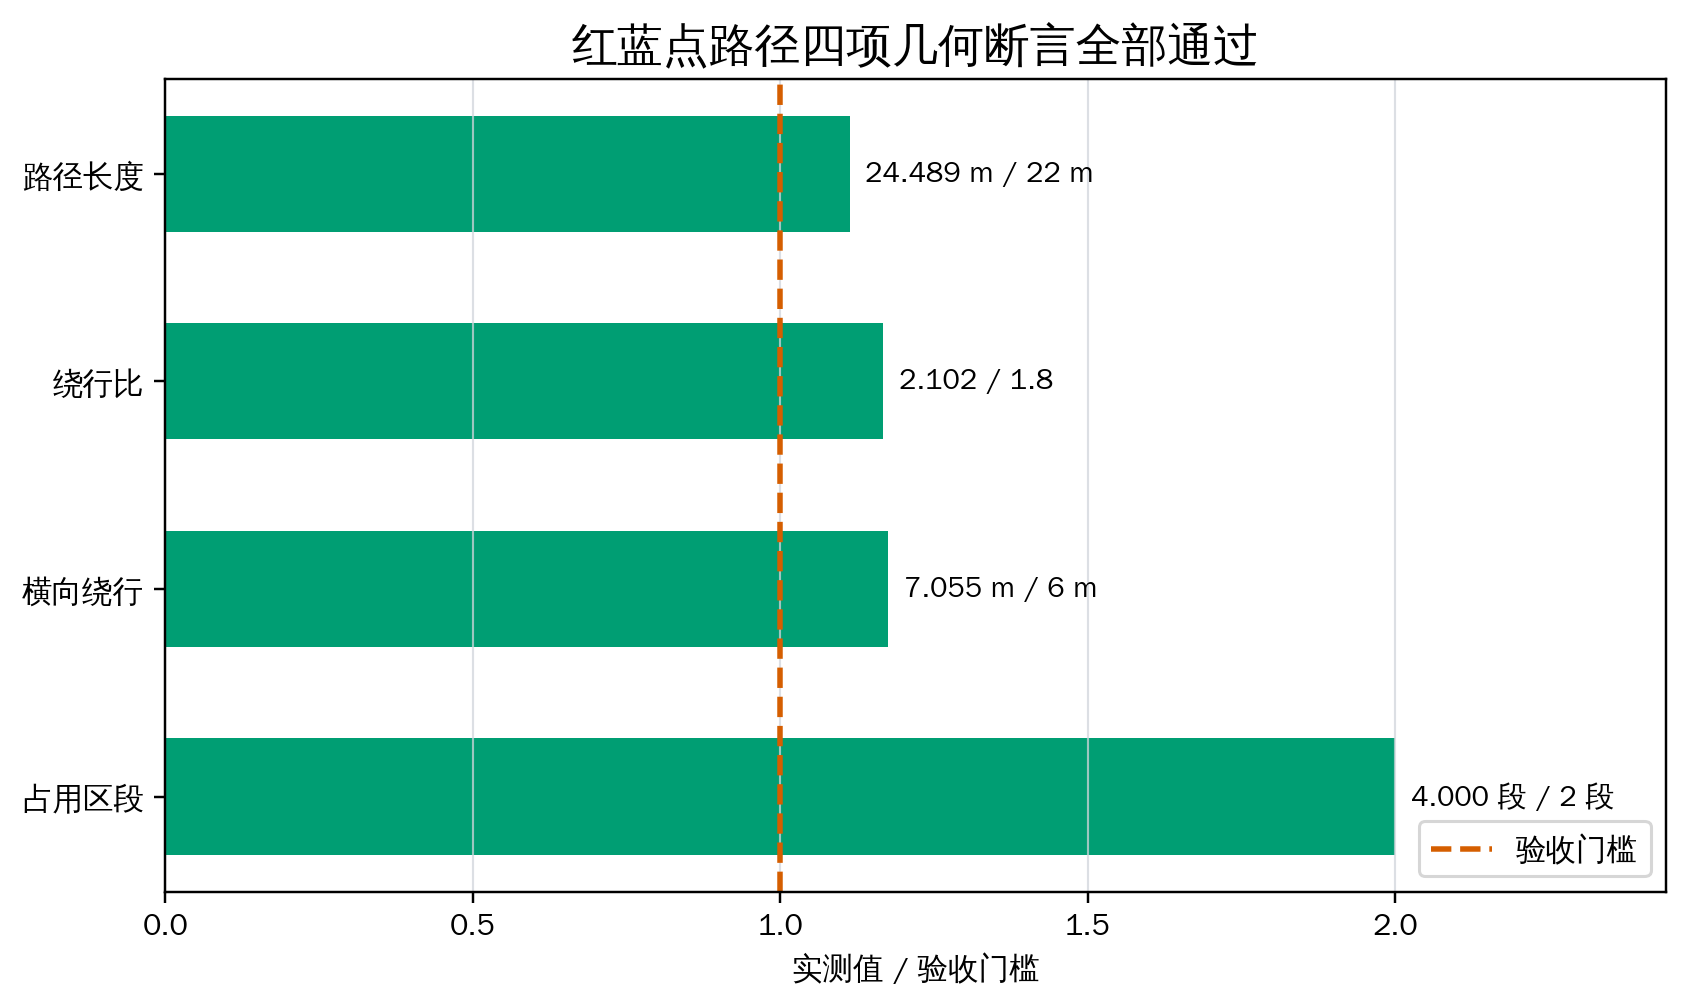
\includegraphics[width=0.94\textwidth]{figures/red_blue_acceptance_metrics.png}
  \caption{图 4：路径四项验收指标相对门槛的通过情况}
\end{figure}

\subsection*{5.4 定位、时钟与运行时数据}

\begin{longtable}{p{5.0cm}p{4.0cm}p{4.0cm}}
  \toprule
  指标 & 实测值 & 结论\\
  \midrule
  \endhead
  静止位置漂移 & 0.000 m & 稳定\\
  静止航向漂移 & 0.000 rad & 稳定\\
  LaserScan/地图匹配率 & 1.000 & 通过\\
  \texttt{/clock} 四窗口平均频率 &
  19.967、19.947、20.002、19.997 Hz & 加载后稳定在约 20 Hz\\
  规划器插件 & \texttt{tb4\_astar\_planner/AStarPlanner} & 正确加载\\
  Nav2 lifecycle & planner/controller/BT 均为 \texttt{active [3]} & 通过\\
  完整视频 & H.264，15 fps，1336.604 s & 覆盖 1248.075 s action\\
  \bottomrule
\end{longtable}

\begin{figure}[H]
  \centering
  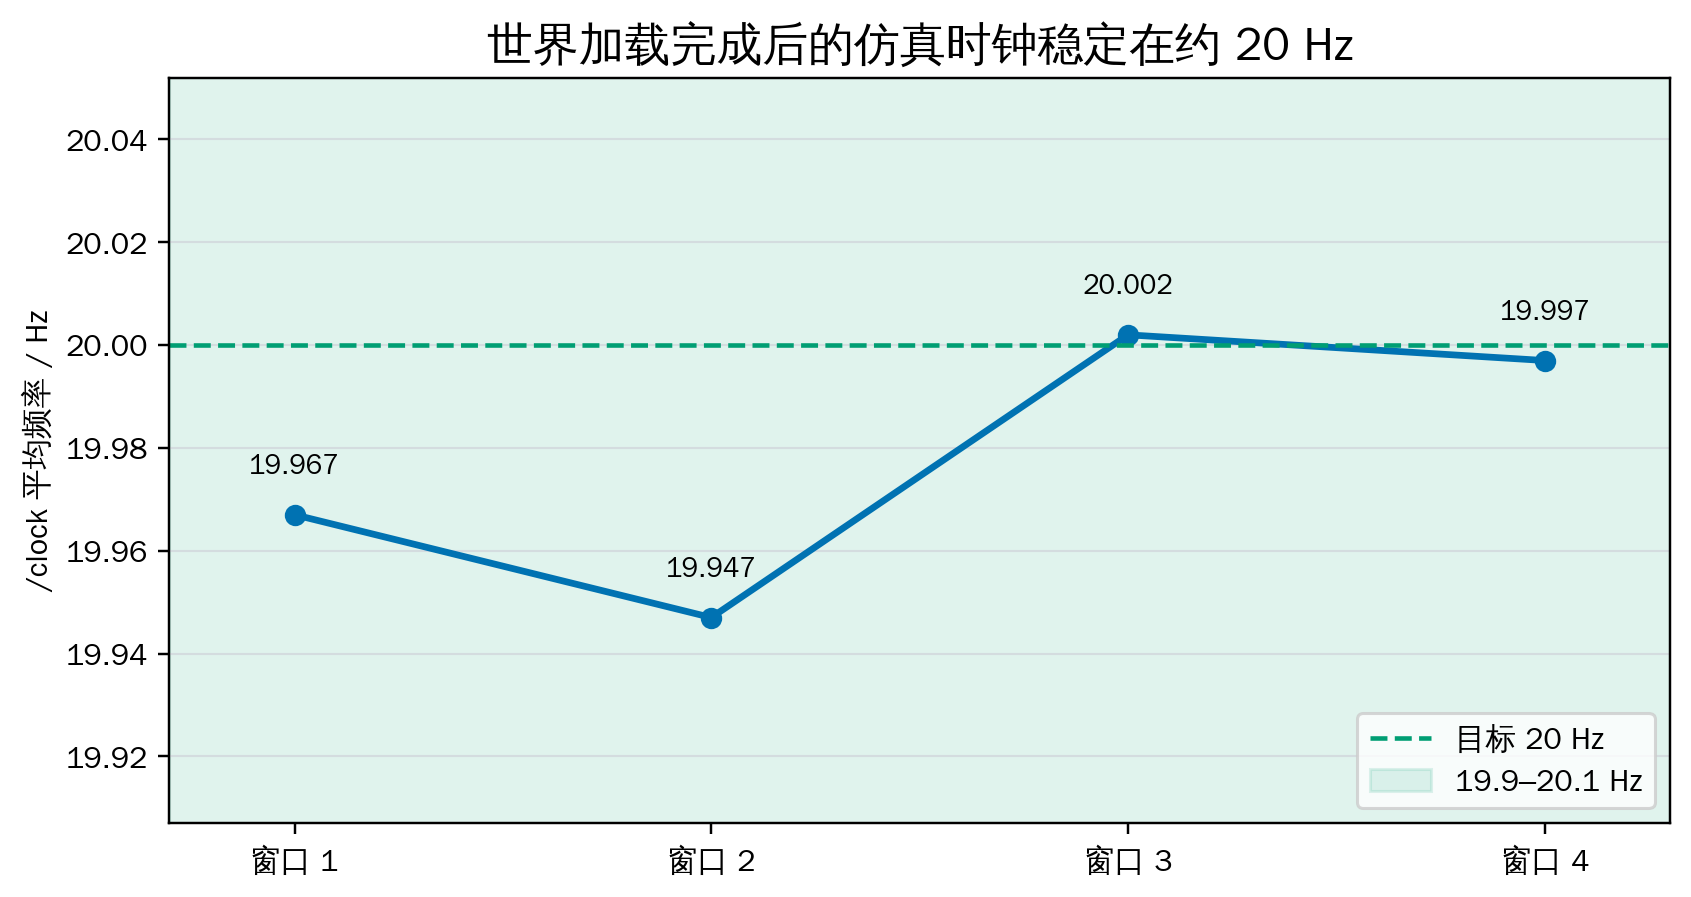
\includegraphics[width=0.94\textwidth]{figures/red_blue_clock_stability.png}
  \caption{图 5：世界加载完成后的仿真时钟频率}
\end{figure}

\begin{figure}[H]
  \centering
  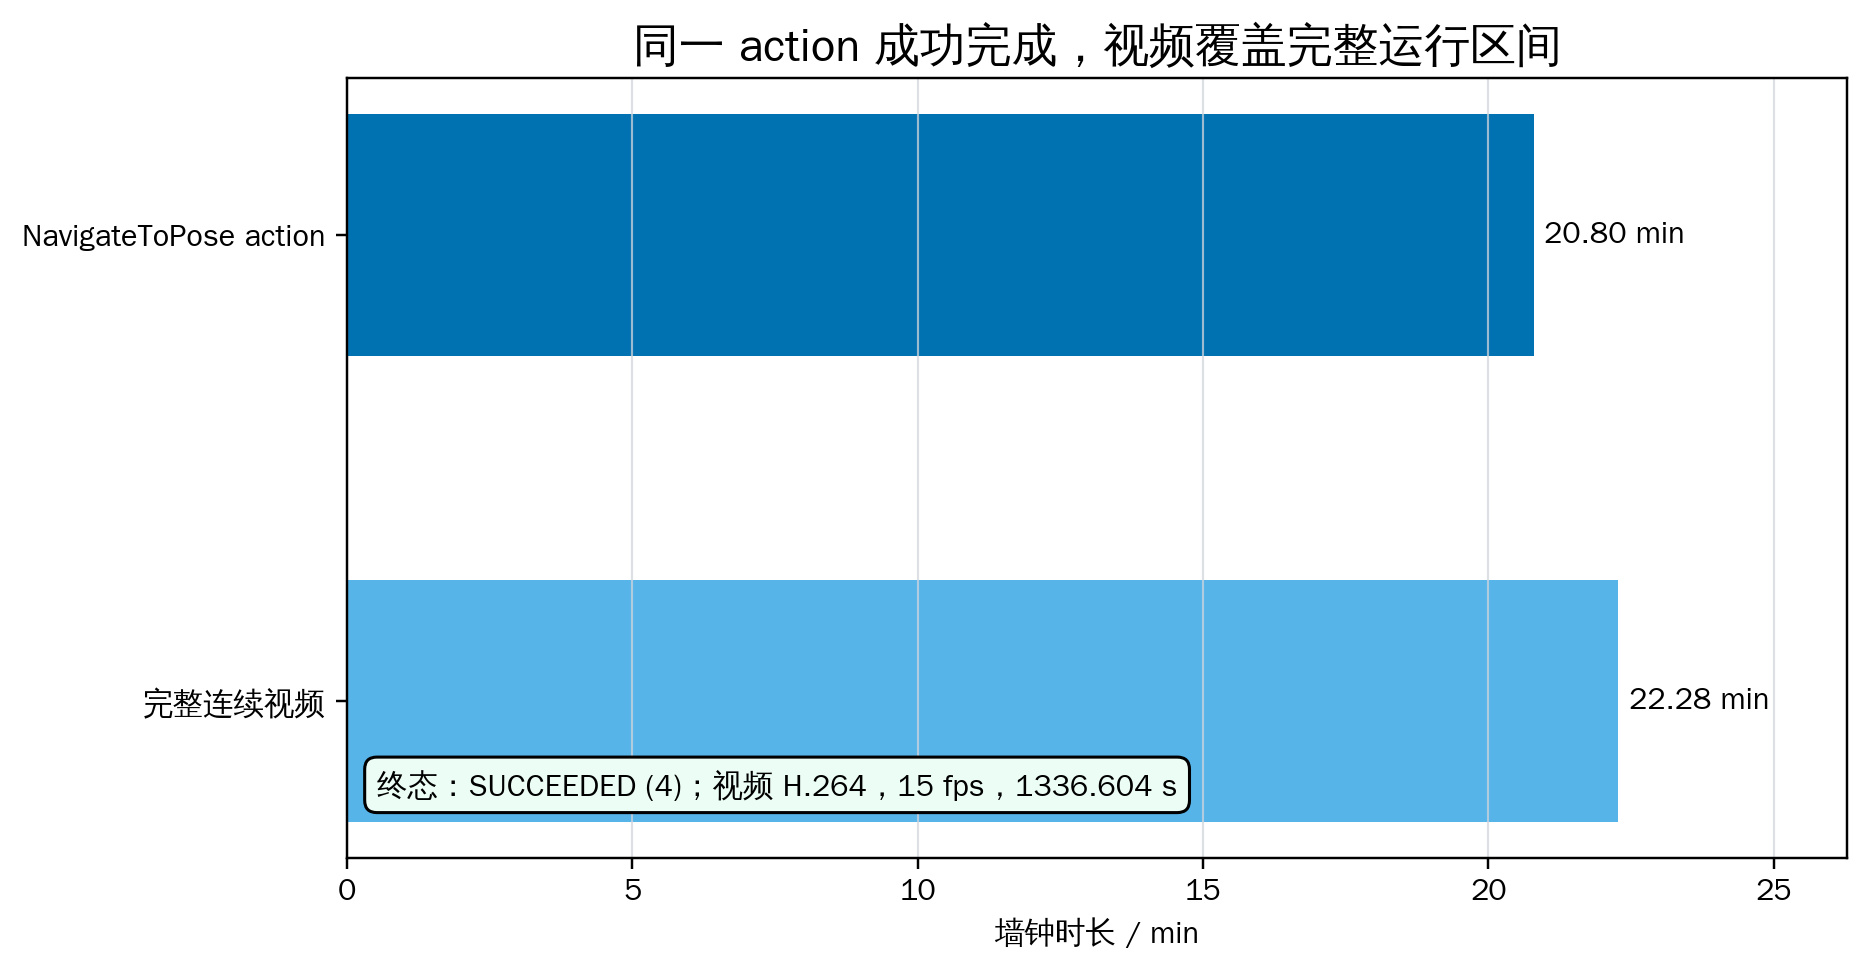
\includegraphics[width=0.94\textwidth]{figures/red_blue_runtime_summary.png}
  \caption{图 6：action 与完整视频时长对比}
\end{figure}

\subsection*{5.5 关键运行截图}

\begin{figure}[H]
  \centering
  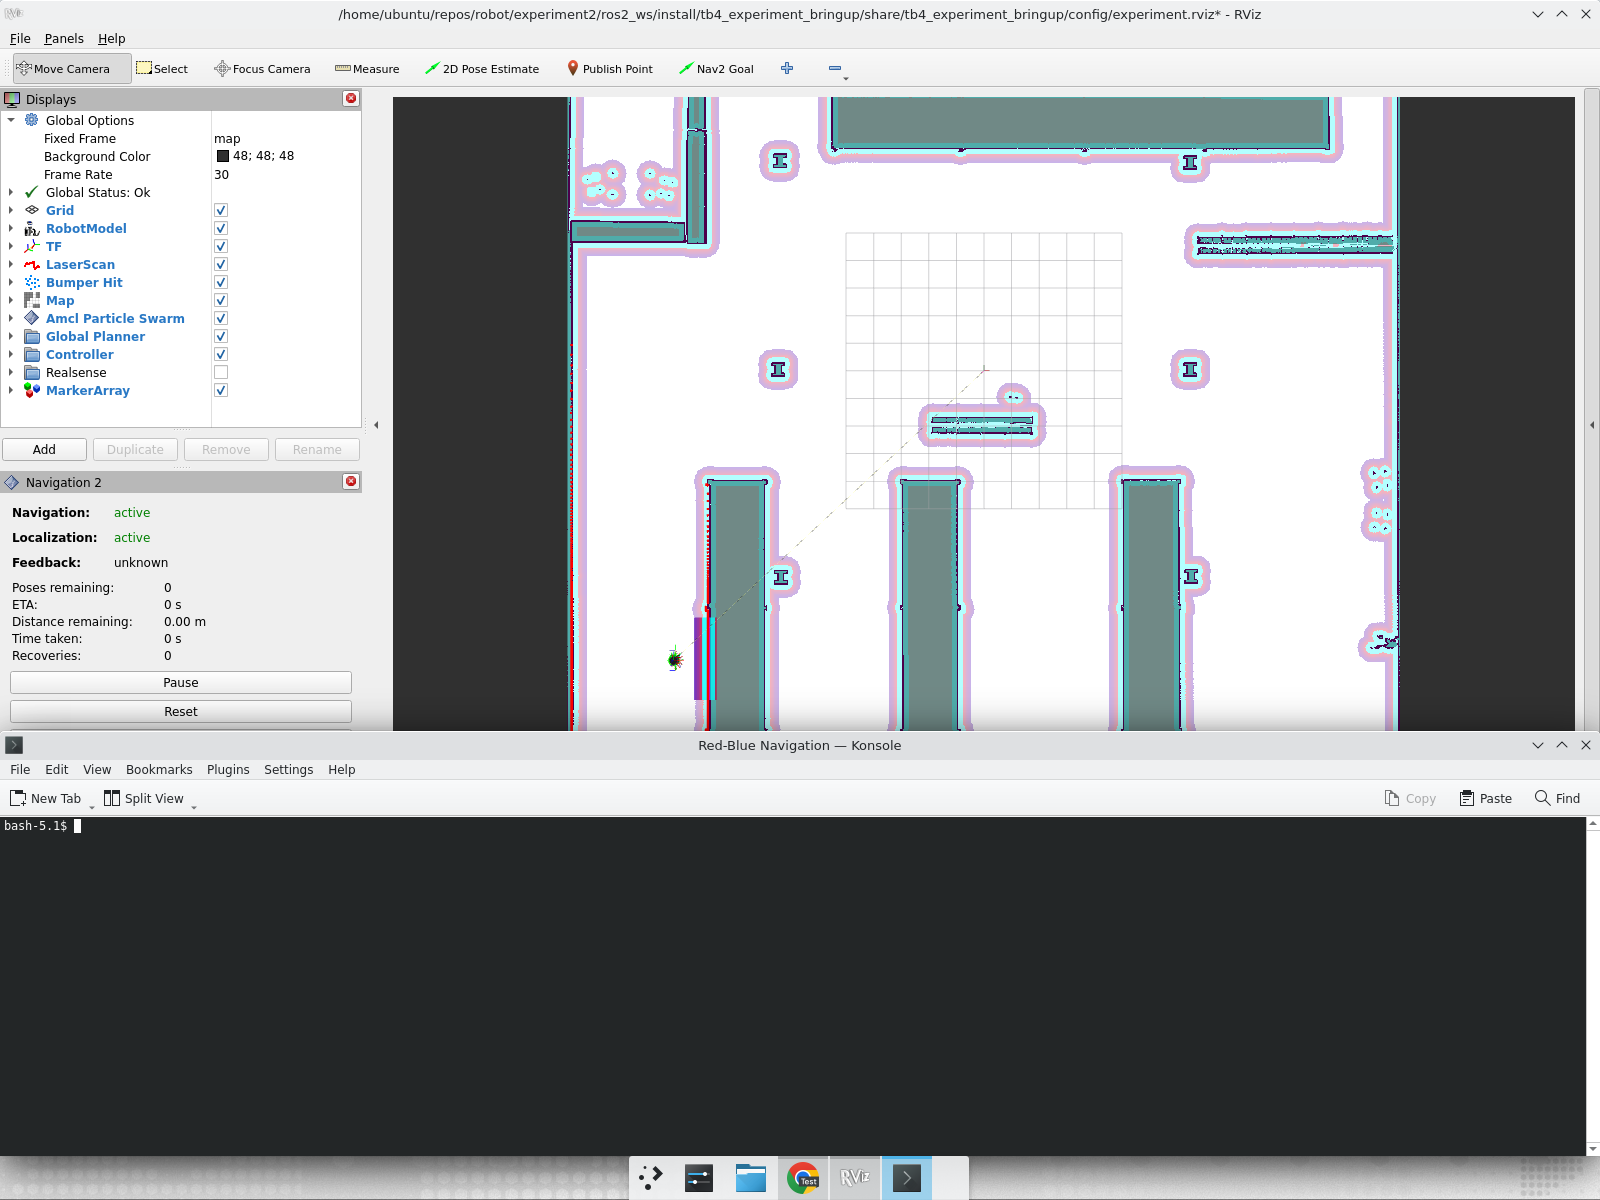
\includegraphics[width=0.92\textwidth]{figures/red_blue_start.png}
  \caption{图 7：红点起始状态：AMCL 已定位并准备发送目标}
\end{figure}

\begin{figure}[H]
  \centering
  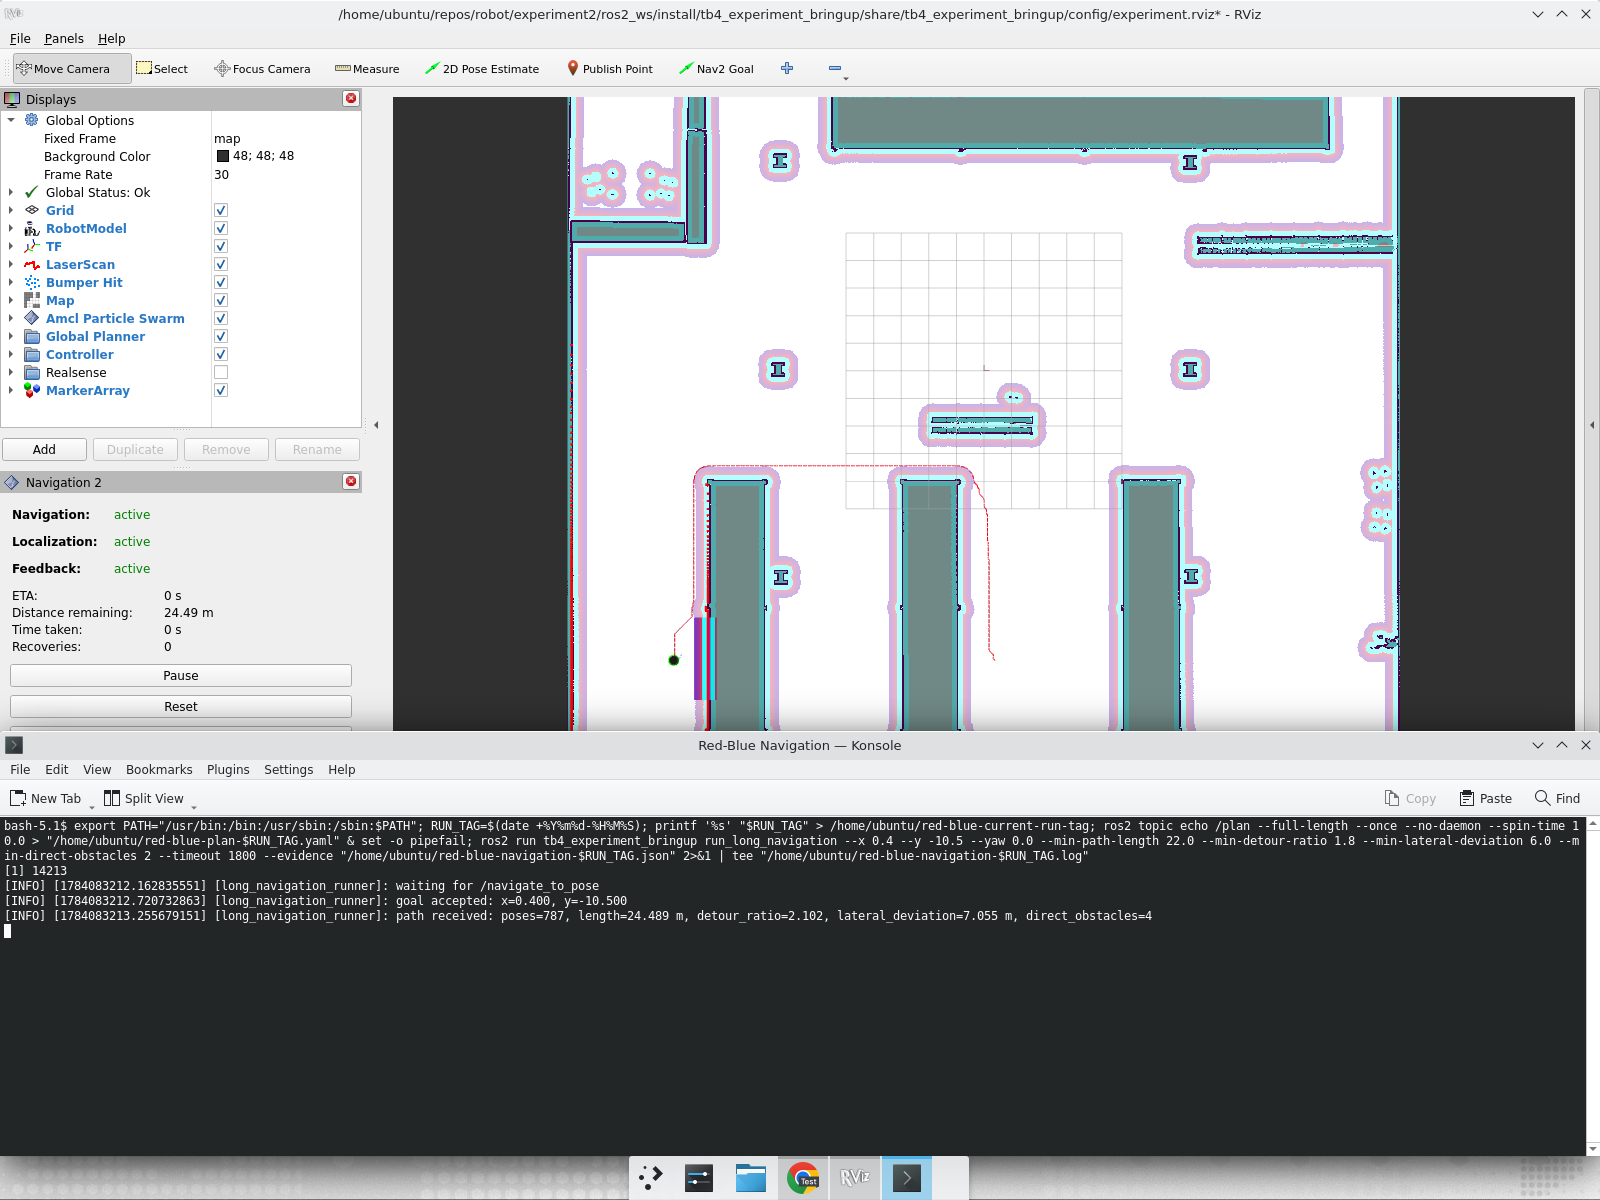
\includegraphics[width=0.92\textwidth]{figures/red_blue_path.png}
  \caption{图 8：RViz 接受的 24.49 m 双货架 A* 全局路径}
\end{figure}

\begin{figure}[H]
  \centering
  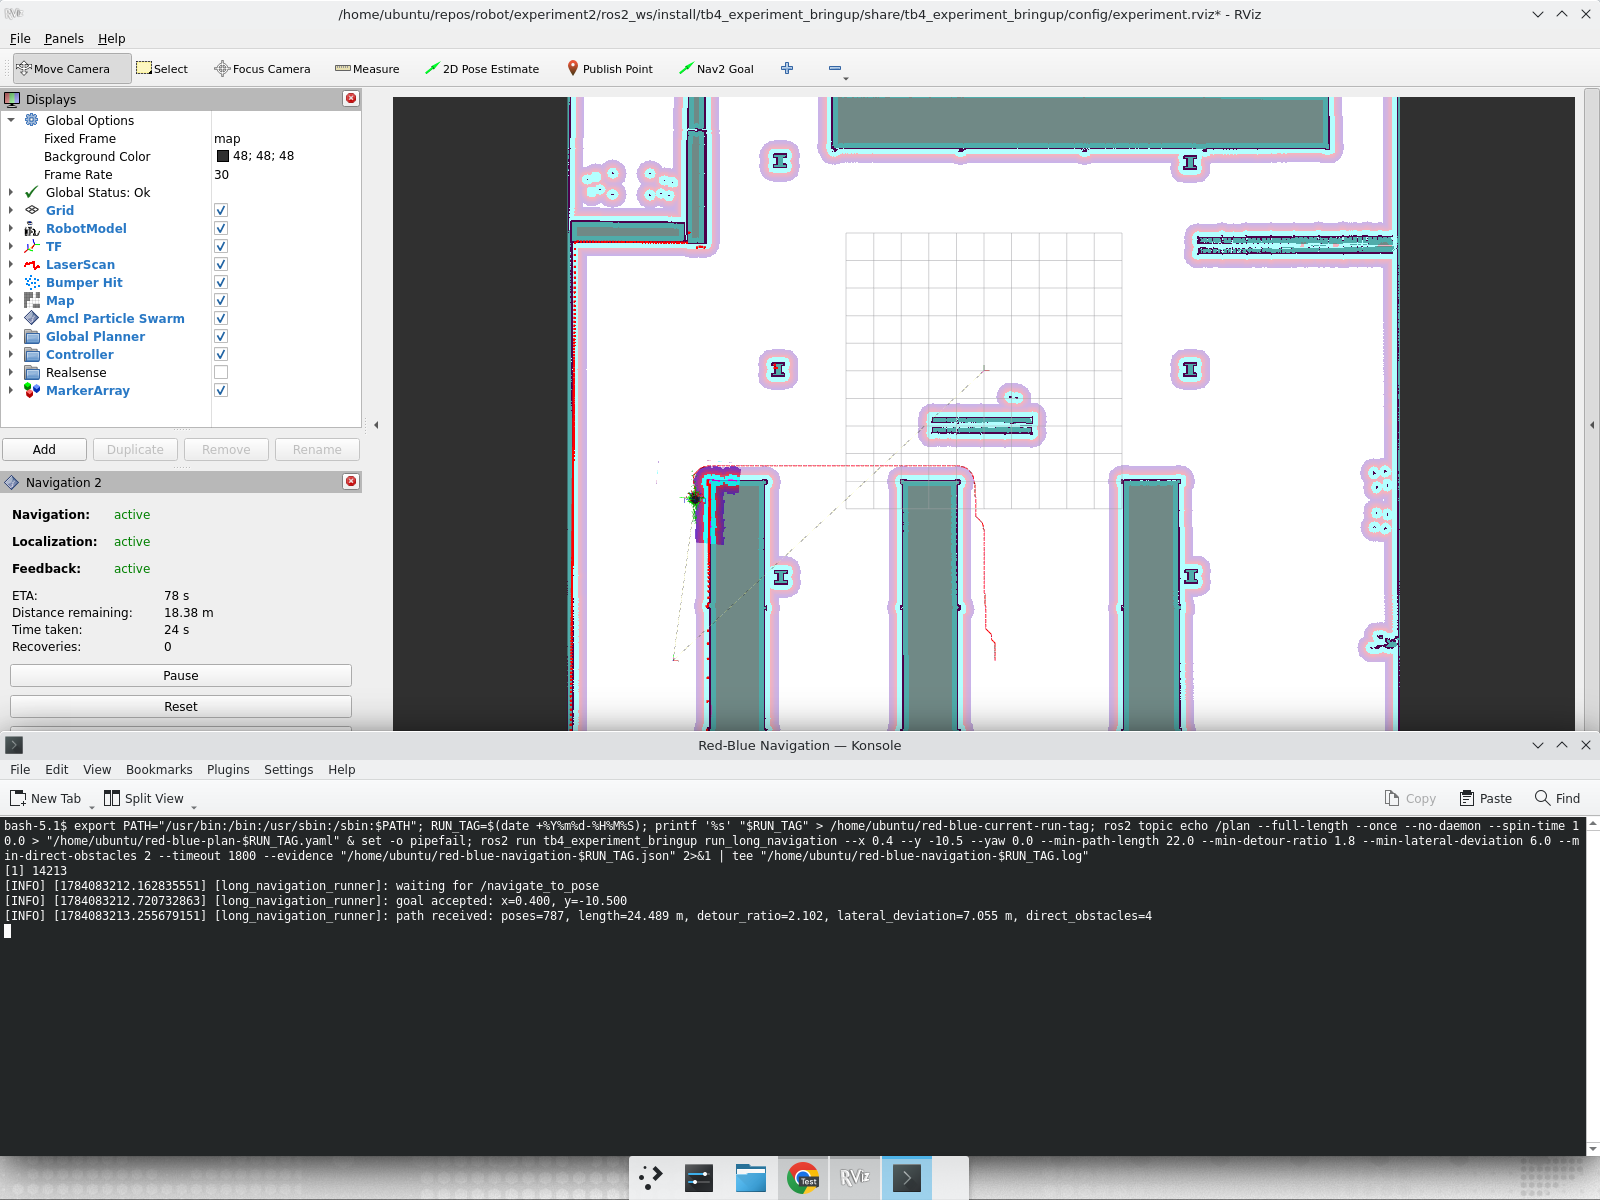
\includegraphics[width=0.92\textwidth]{figures/red_blue_first_shelf.png}
  \caption{图 9：机器人已绕过第一组货架端部，剩余距离 18.38 m}
\end{figure}

\begin{figure}[H]
  \centering
  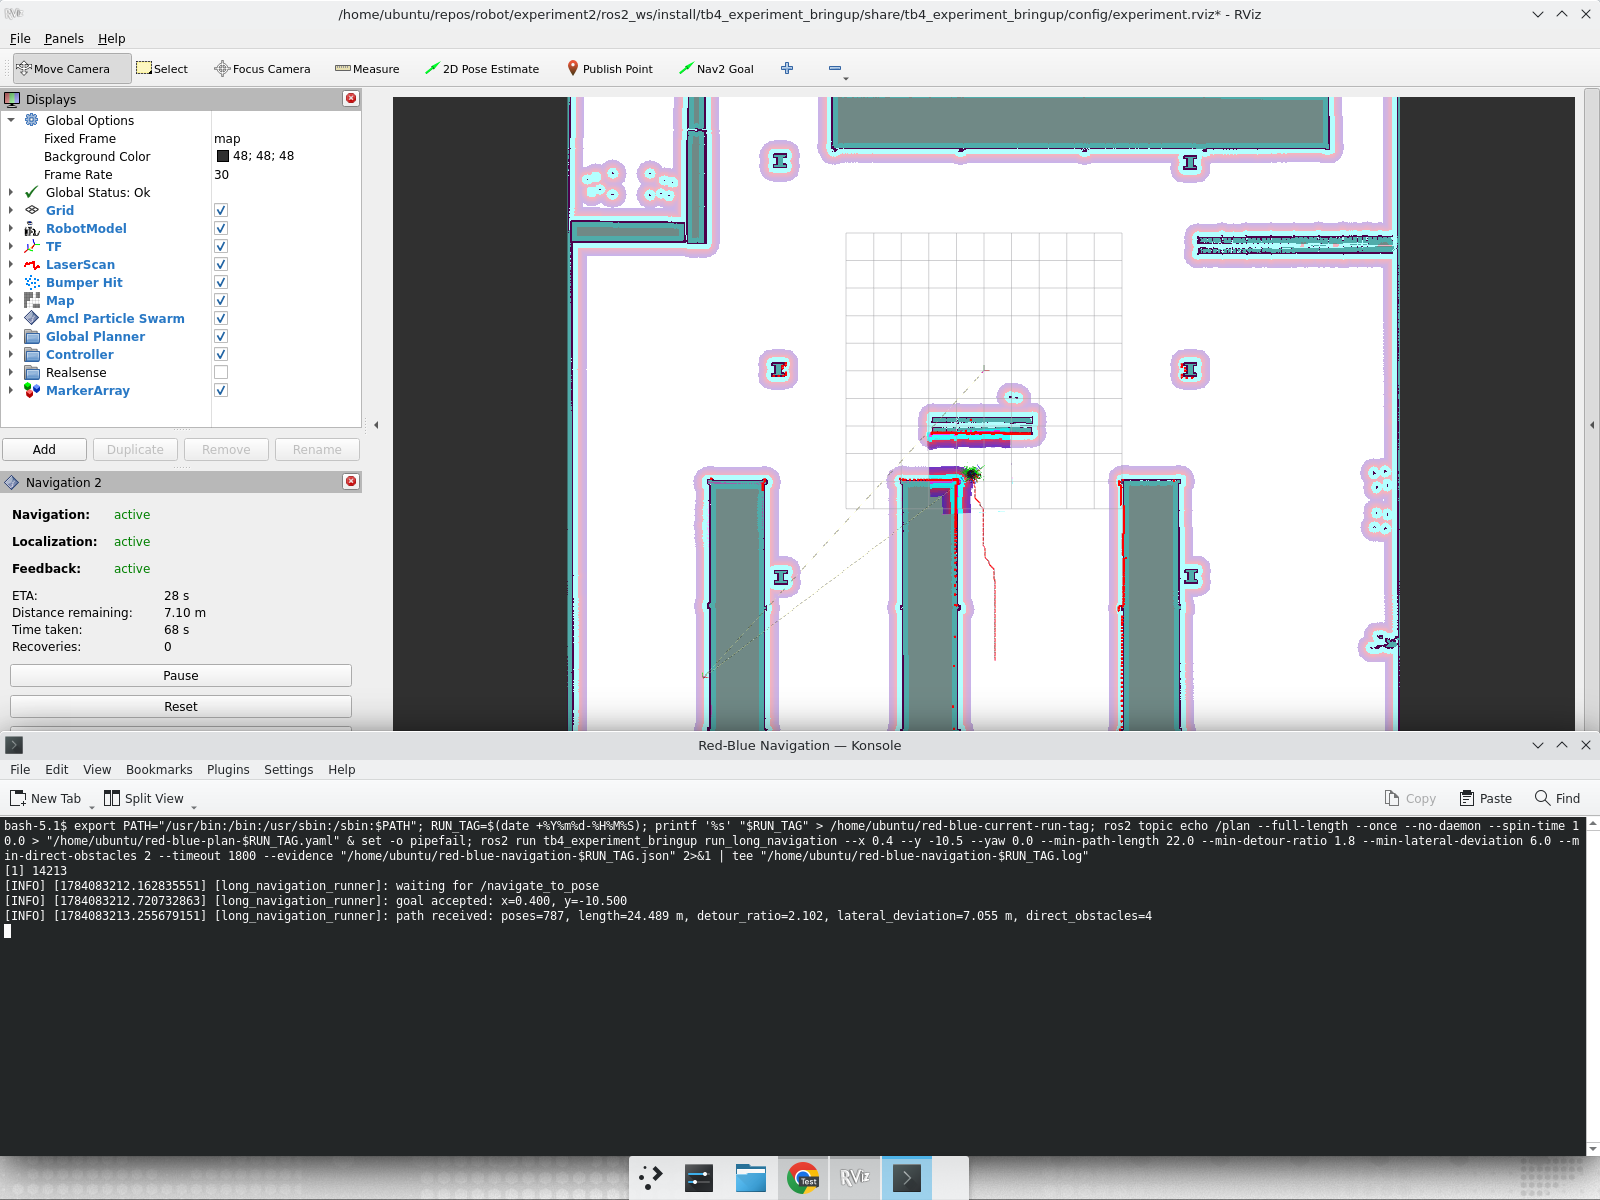
\includegraphics[width=0.92\textwidth]{figures/red_blue_second_shelf.png}
  \caption{图 10：机器人已绕过第二组货架端部，剩余距离 7.10 m}
\end{figure}

\begin{figure}[H]
  \centering
  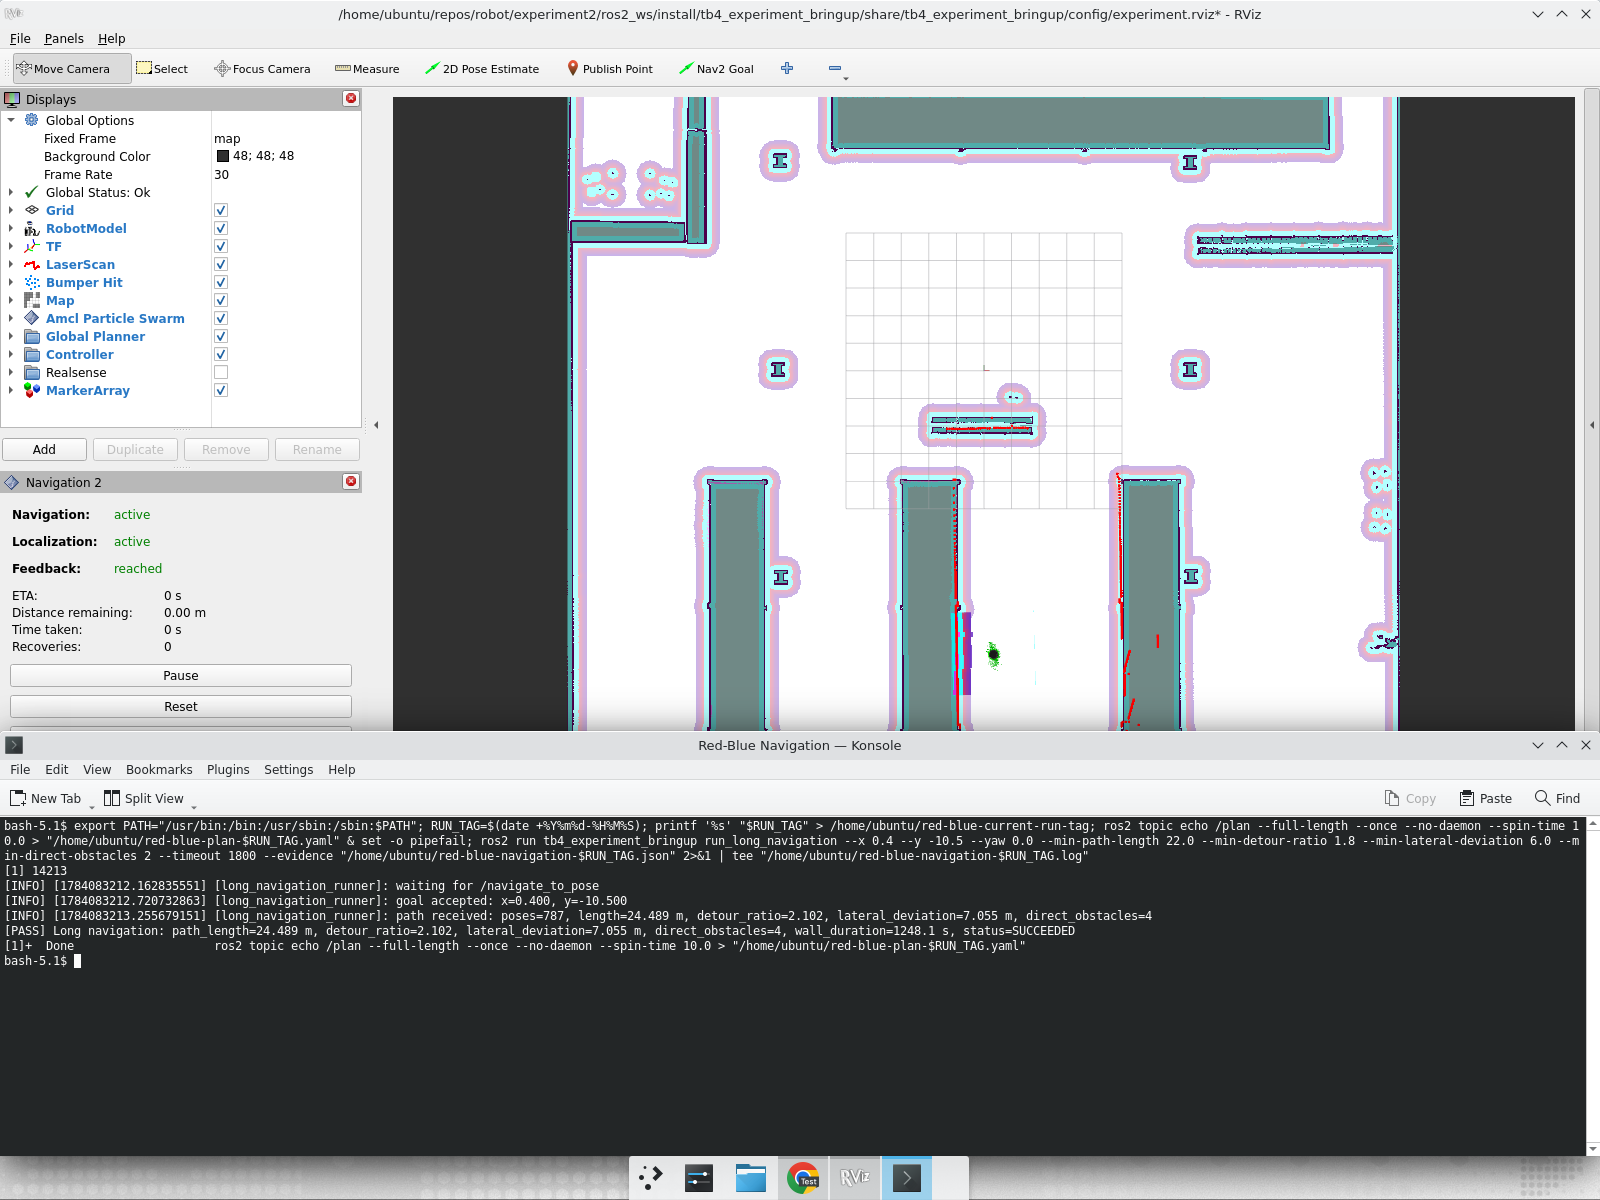
\includegraphics[width=0.92\textwidth]{figures/red_blue_success.png}
  \caption{图 11：蓝点终态：同一 action 返回 SUCCEEDED (4)}
\end{figure}

\subsection*{5.6 实地建图与导航证据}

实地实验在实体 TurtleBot4（ROS 2 Humble / Ubuntu 22.04）上完成了 SLAM 增量
建图、地图保存与自主导航，过程整体进展顺利。本部分以两项辅助证据说明完成
情况：（1）实地 SLAM 保存的占据栅格地图（图 2），尺寸为 $296\times494$ 个栅
格，可辨识出房间、走廊等结构轮廓；（2）实地建图与自主导航的连续录像
（\texttt{video/实验二-实地导航.mp4}）。与仿真部分不同，实地实验未导出可复算的
路径 YAML、rosbag 与 action 终态 JSON，因此本节不给出实地路径长度、终点误差等
量化数值，而以地图与录像作为功能完成的佐证，量化验收继续以仿真部分为主。

\section*{六、实验结果与分析（必填）}

\subsection*{6.1 仿真任务完成度}

本次仿真完成了从红点到蓝点的完整闭环导航。原始路径、运行日志和 JSON 对同一条
路线给出了完全一致的 787 个位姿和 24.488843 m 路径长度。路径的四项几何指标均
超过门槛，直线穿过 4 段占用区，而 A* 路径通过两个货架端部绕行，最终同一
\texttt{NavigateToPose} action 返回 \texttt{SUCCEEDED (4)}。因此实验同时证明了
规划器加载、全局路径生成、局部控制、避障和目标到达，而非仅证明离线算法能够
输出坐标序列。

\subsection*{6.2 A* 路径合理性}

路径长度比最低要求高 2.489 m，绕行比比最低要求高 0.302，最大横向绕行比最低
要求高 1.055 m，直线障碍段数是最低要求的两倍。四项指标共同排除了“目标点足够
接近”“直线路径没有实质障碍”以及“仅绕过单个货架边缘”等弱验收情形。

规划器在膨胀代价上施加惩罚，因此优化目标并非纯粹最短几何距离。24.489 m 路径
相对于 11.650 m 直线距离显著增加，但换取了对致命栅格、未知区域和货架膨胀区的
规避。对于课程要求的自主绕障演示，这种代价感知结果比贴边最短路径更具安全性。

\subsection*{6.3 定位与仿真时钟}

定位检查记录的位置和航向漂移均为零，LaserScan/地图匹配率为 1.000，说明目标发送
前的静止定位状态一致。该结果只能证明当前 15 s 窗口和仿真传感器条件下的稳定性，
不能等同于实体机器人在轮滑、反光、遮挡或动态人群条件下的定位精度。

启动校验器在重载世界初始化阶段检测到过一次 \texttt{/clock} 间隙；实验在加载完成后
重新采样，四个窗口均接近 20 Hz。报告保留该异常而不删除，说明启动瞬态和稳定运行
阶段应分开评价。

\subsection*{6.4 连续视频与 action 证据}

完整视频时长为 1336.604 s，比 action 墙钟时长长 88.529 s，能够覆盖目标发送前的
准备、完整运动和终态确认。视频为 H.264、15 fps，并带有字幕流。40.709 s 的浓缩
摘要没有被用于功能验收，从而避免通过加速或删减掩盖中途停滞、碰撞或人工接管。

\subsection*{6.5 结果的适用边界}

\begin{enumerate}[label=\arabic*)]
  \item VMware 使用 server-only Gazebo、软件渲染、降低传感器频率和较低实时因子，
  运行时长不代表标准主机性能；
  \item 仿真地图、摩擦、激光噪声和底盘模型不能完整复现实体环境；
  \item 静止定位稳定不代表运动过程中的全局定位误差；
  \item 路径几何验收证明了仿真规划难度；
  \item 实地实验以连续录像和保存的栅格地图佐证建图与导航的完成，量化指标仍以
  仿真部分为主。
\end{enumerate}

\subsection*{6.6 实地实验小结}

实地实验将仿真中验证的 ROS 2 工作空间、A* 规划器插件和 Nav2 参数部署到实体
TurtleBot4，完成了实地 SLAM 增量建图、地图保存与自主导航，整体进展顺利。保存的
栅格地图（图 2）结构清晰，配合连续导航录像共同证明实地建图与自主移动均已实现。
本次实地实验以视频和地图作为辅助佐证，与仿真部分的量化验收互为补充。

\section*{七、讨论、心得}

本实验表明，移动机器人自主导航的难点不只在于实现 A* 搜索本身。算法必须通过
pluginlib 生命周期接入 Nav2，使用实时 costmap，并与 AMCL、TF、行为树、局部控制器
和速度平滑器共同工作。即使路径几何正确，仿真时钟停滞、定位尚未收敛、lifecycle
激活顺序或传感器频率异常仍可能导致整条 action 失败。

通过为路径长度、绕行比、横向绕行和直线障碍段数设置独立门槛，可以把“看起来绕过
了障碍”转化为可重复计算的结论。保存完整 YAML、JSON 和日志后，报告中的关键数值
可以从原始数据重新计算，而不是依赖人工抄录。完整原速视频进一步补充了数据文件
无法证明的连续运动和无人工接管过程。

将同一套算法与参数部署到实体 TurtleBot4 后，实地 SLAM 建图、地图保存与自主导航
均顺利完成，保存的栅格地图与连续录像共同佐证了从仿真到实地的迁移效果。实地实验
表明本工作空间具有良好的可移植性，仿真中验证的规划与定位流程能够在真实机器人
上复现。

\section*{参考文献}

\begin{enumerate}[label={[\arabic*]}]
  \item S. M. LaValle. \emph{Planning Algorithms}. Cambridge University Press, 2006.
  \item S. Thrun, W. Burgard, D. Fox. \emph{Probabilistic Robotics}. MIT Press, 2005.
  \item Open Navigation LLC. Nav2 Documentation.
  \url{https://docs.nav2.org/}.
  \item Clearpath Robotics. TurtleBot 4 User Manual.
  \url{https://turtlebot.github.io/turtlebot4-user-manual/}.
  \item ROS 2 Documentation: Humble Hawksbill.
  \url{https://docs.ros.org/en/humble/}.
  \item SLAM Toolbox Documentation.
  \url{https://github.com/SteveMacenski/slam_toolbox}.
\end{enumerate}

\appendix
\section*{附录 A：仿真验收命令}

\begin{verbatim}
ros2 topic hz /clock
ros2 run tb4_experiment_bringup validate_localization_stability
ros2 param get /planner_server planner_plugins
ros2 param get /planner_server GridBased.plugin
ros2 lifecycle get /planner_server
ros2 lifecycle get /controller_server
ros2 lifecycle get /bt_navigator
ros2 run tb4_experiment_bringup run_long_navigation \
  --x 0.4 --y -10.5 \
  --min-path-length 22.0 \
  --min-detour-ratio 1.8 \
  --min-lateral-deviation 6.0 \
  --min-direct-obstacles 2 \
  --timeout 1800
\end{verbatim}

\end{document}
